% The first argument is the \documentclass, which tells latex which template
% we're using to build this document. It's usually safe to just use "article".
\documentclass{article}

% include some packages...
\usepackage{fullpage} % change settings for a smaller margin
\usepackage{graphicx} % gives access to the \includegraphics commands
\usepackage{amsfonts}
\usepackage{float}
\usepackage{enumitem}
\usepackage{caption}
\usepackage[export]{adjustbox}
\usepackage{bookmark}
\graphicspath{{./images/}}

% tell Latex to use no paragraph indentation, but leave some space between
% paragraphs 
\setlength{\parindent}{0in}
\setlength{\parskip}{0.1in}

\newcommand{\tib}[1]{\textit{\textbf{#1}}}
\newcommand{\code}[1]{\texttt{#1}}

% these commands merely set the values for the title/date/author; they don't put
% them in the document... see \maketitle below
\title{CS Department Automated Information Timeline \\ Assignment 4.1: Activity Diagram and Sequence Diagram}
\date{\today}
\author{Matthew Hays, Pawan Bhandari, Sarah Faron, Tim Klimpel}

% all document content goes between \begin{document} and \end{document}
\begin{document}

% this command actually creates the title/date/author in the document
\maketitle
\newpage
\tableofcontents
\listoffigures
\newpage

\section{Introduction}
\subsection{Purpose}
The purpose of this assignment is to work as a team and collaboratively develop a activity diagram for "Create Event" activity. Team members also contributed to create sequence diagrams for two use cases each. The team met multiple times over the course of a few days to work together and come to the final activity diagram presented in section 2 of this document. The sequence diagrams are located in the third section.

\section{Activity Diagram: Create Event}
\begin{figure}[H]
    \centering
    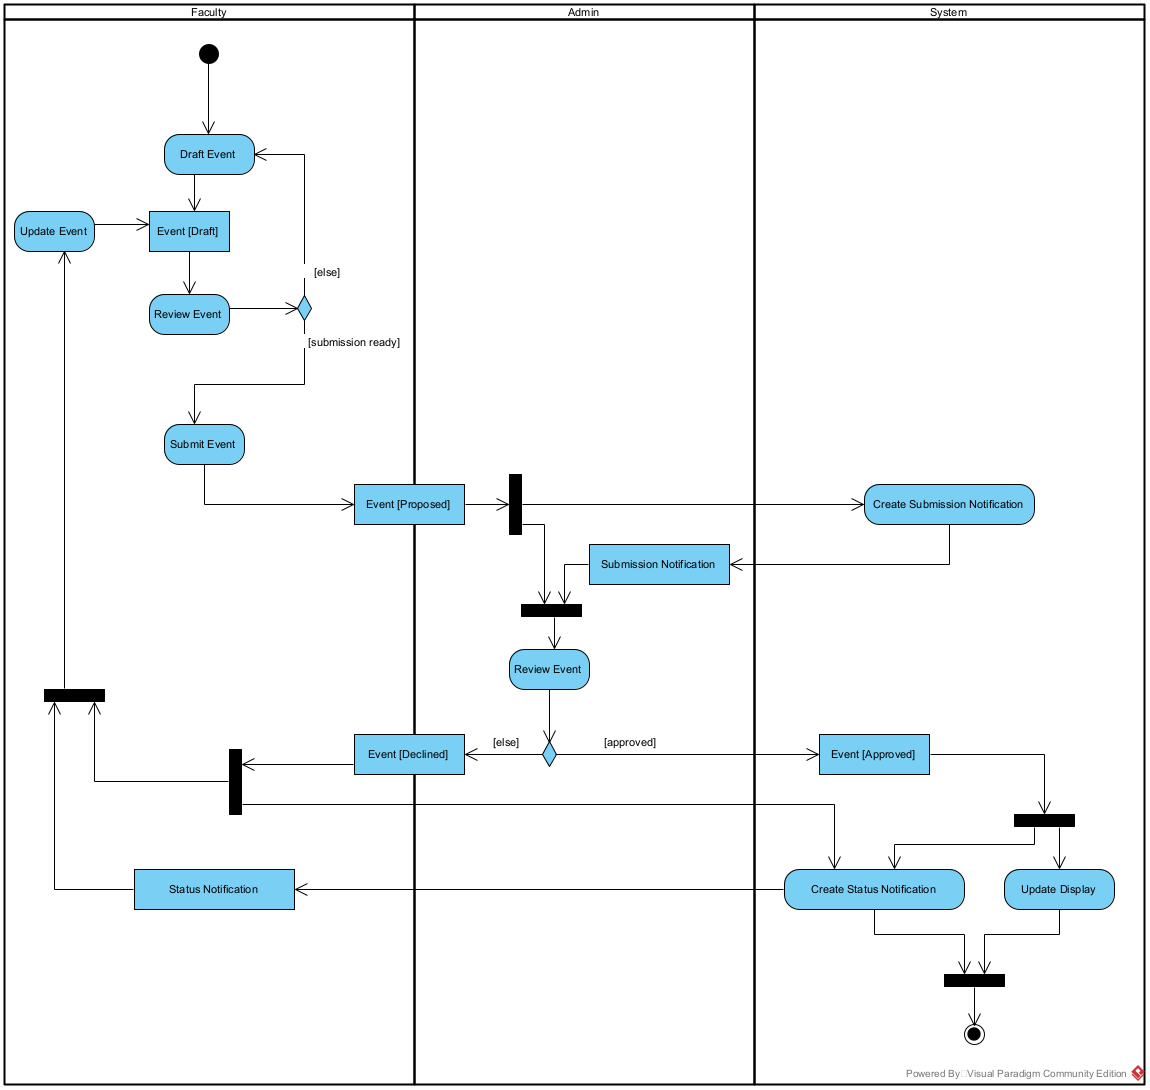
\includegraphics[width=.98\textwidth]{images/activityDiagram-CreateEvent.png}
    \centering
    \caption{Activity Diagram: Create Event}
    \label{fig:activityDiagram}
\end{figure}

\section{Sequence Diagrams}
\subsection{UC04: Create Event (Matthew Hays)}
\begin{figure}[H]
    \centering
    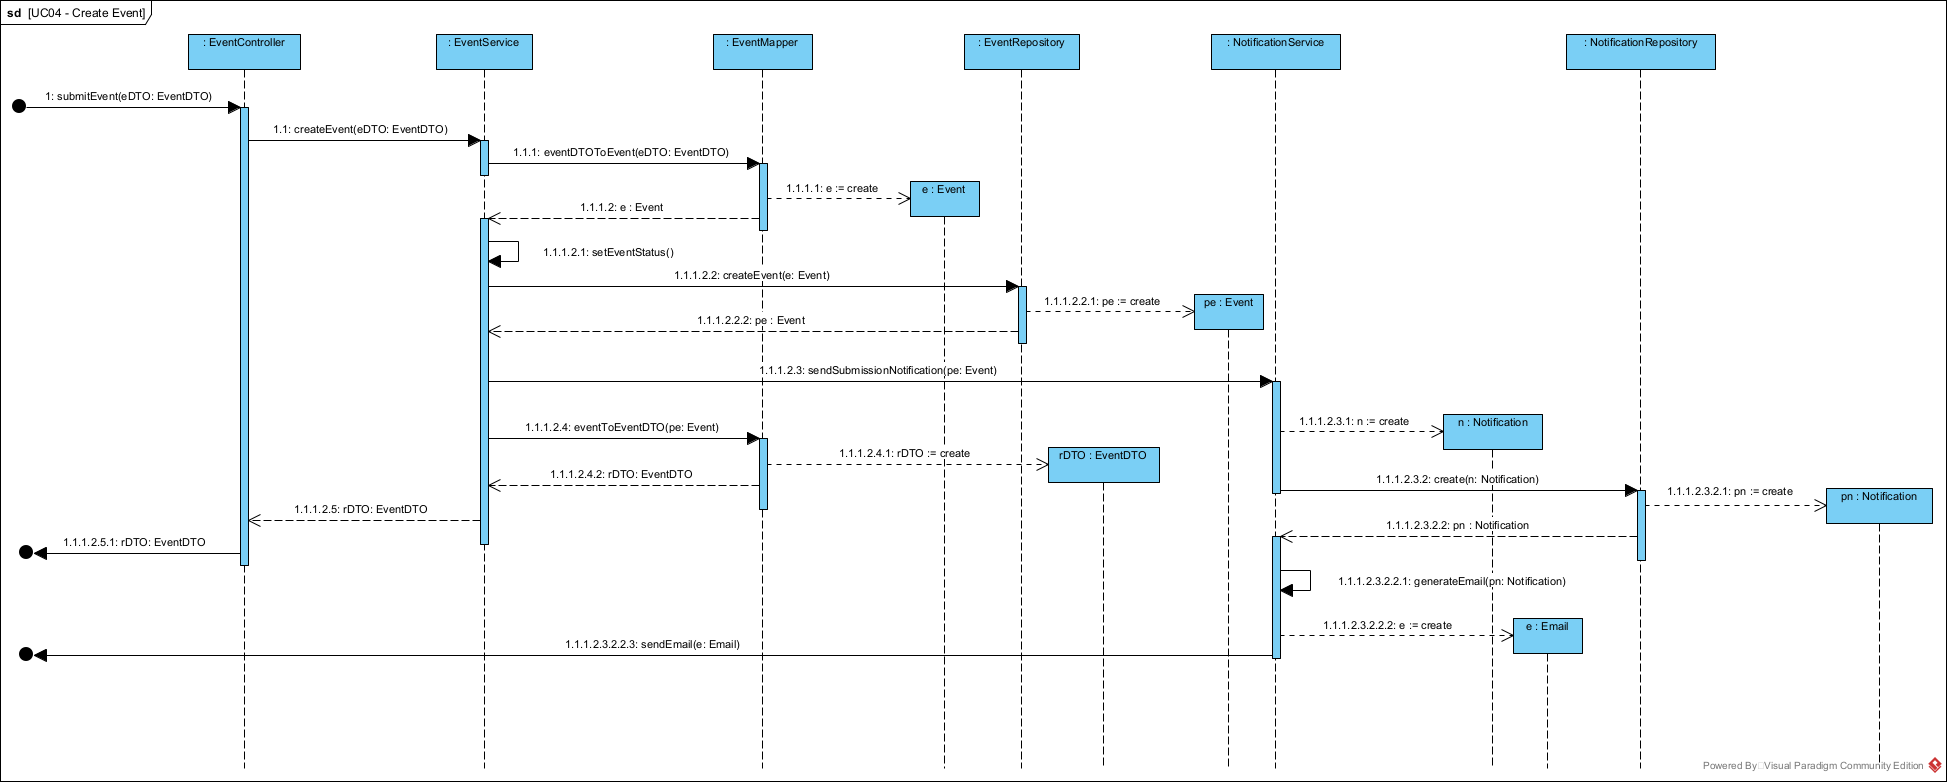
\includegraphics[width=.98\textwidth]{images/SD-UC04-CreateEvent.png}
    \centering
    \caption{Sequence Diagram: Create Event}
\end{figure}
\subsection{UC09: Review for Approvals (Matthew Hays)}
\begin{figure}[H]
    \centering
    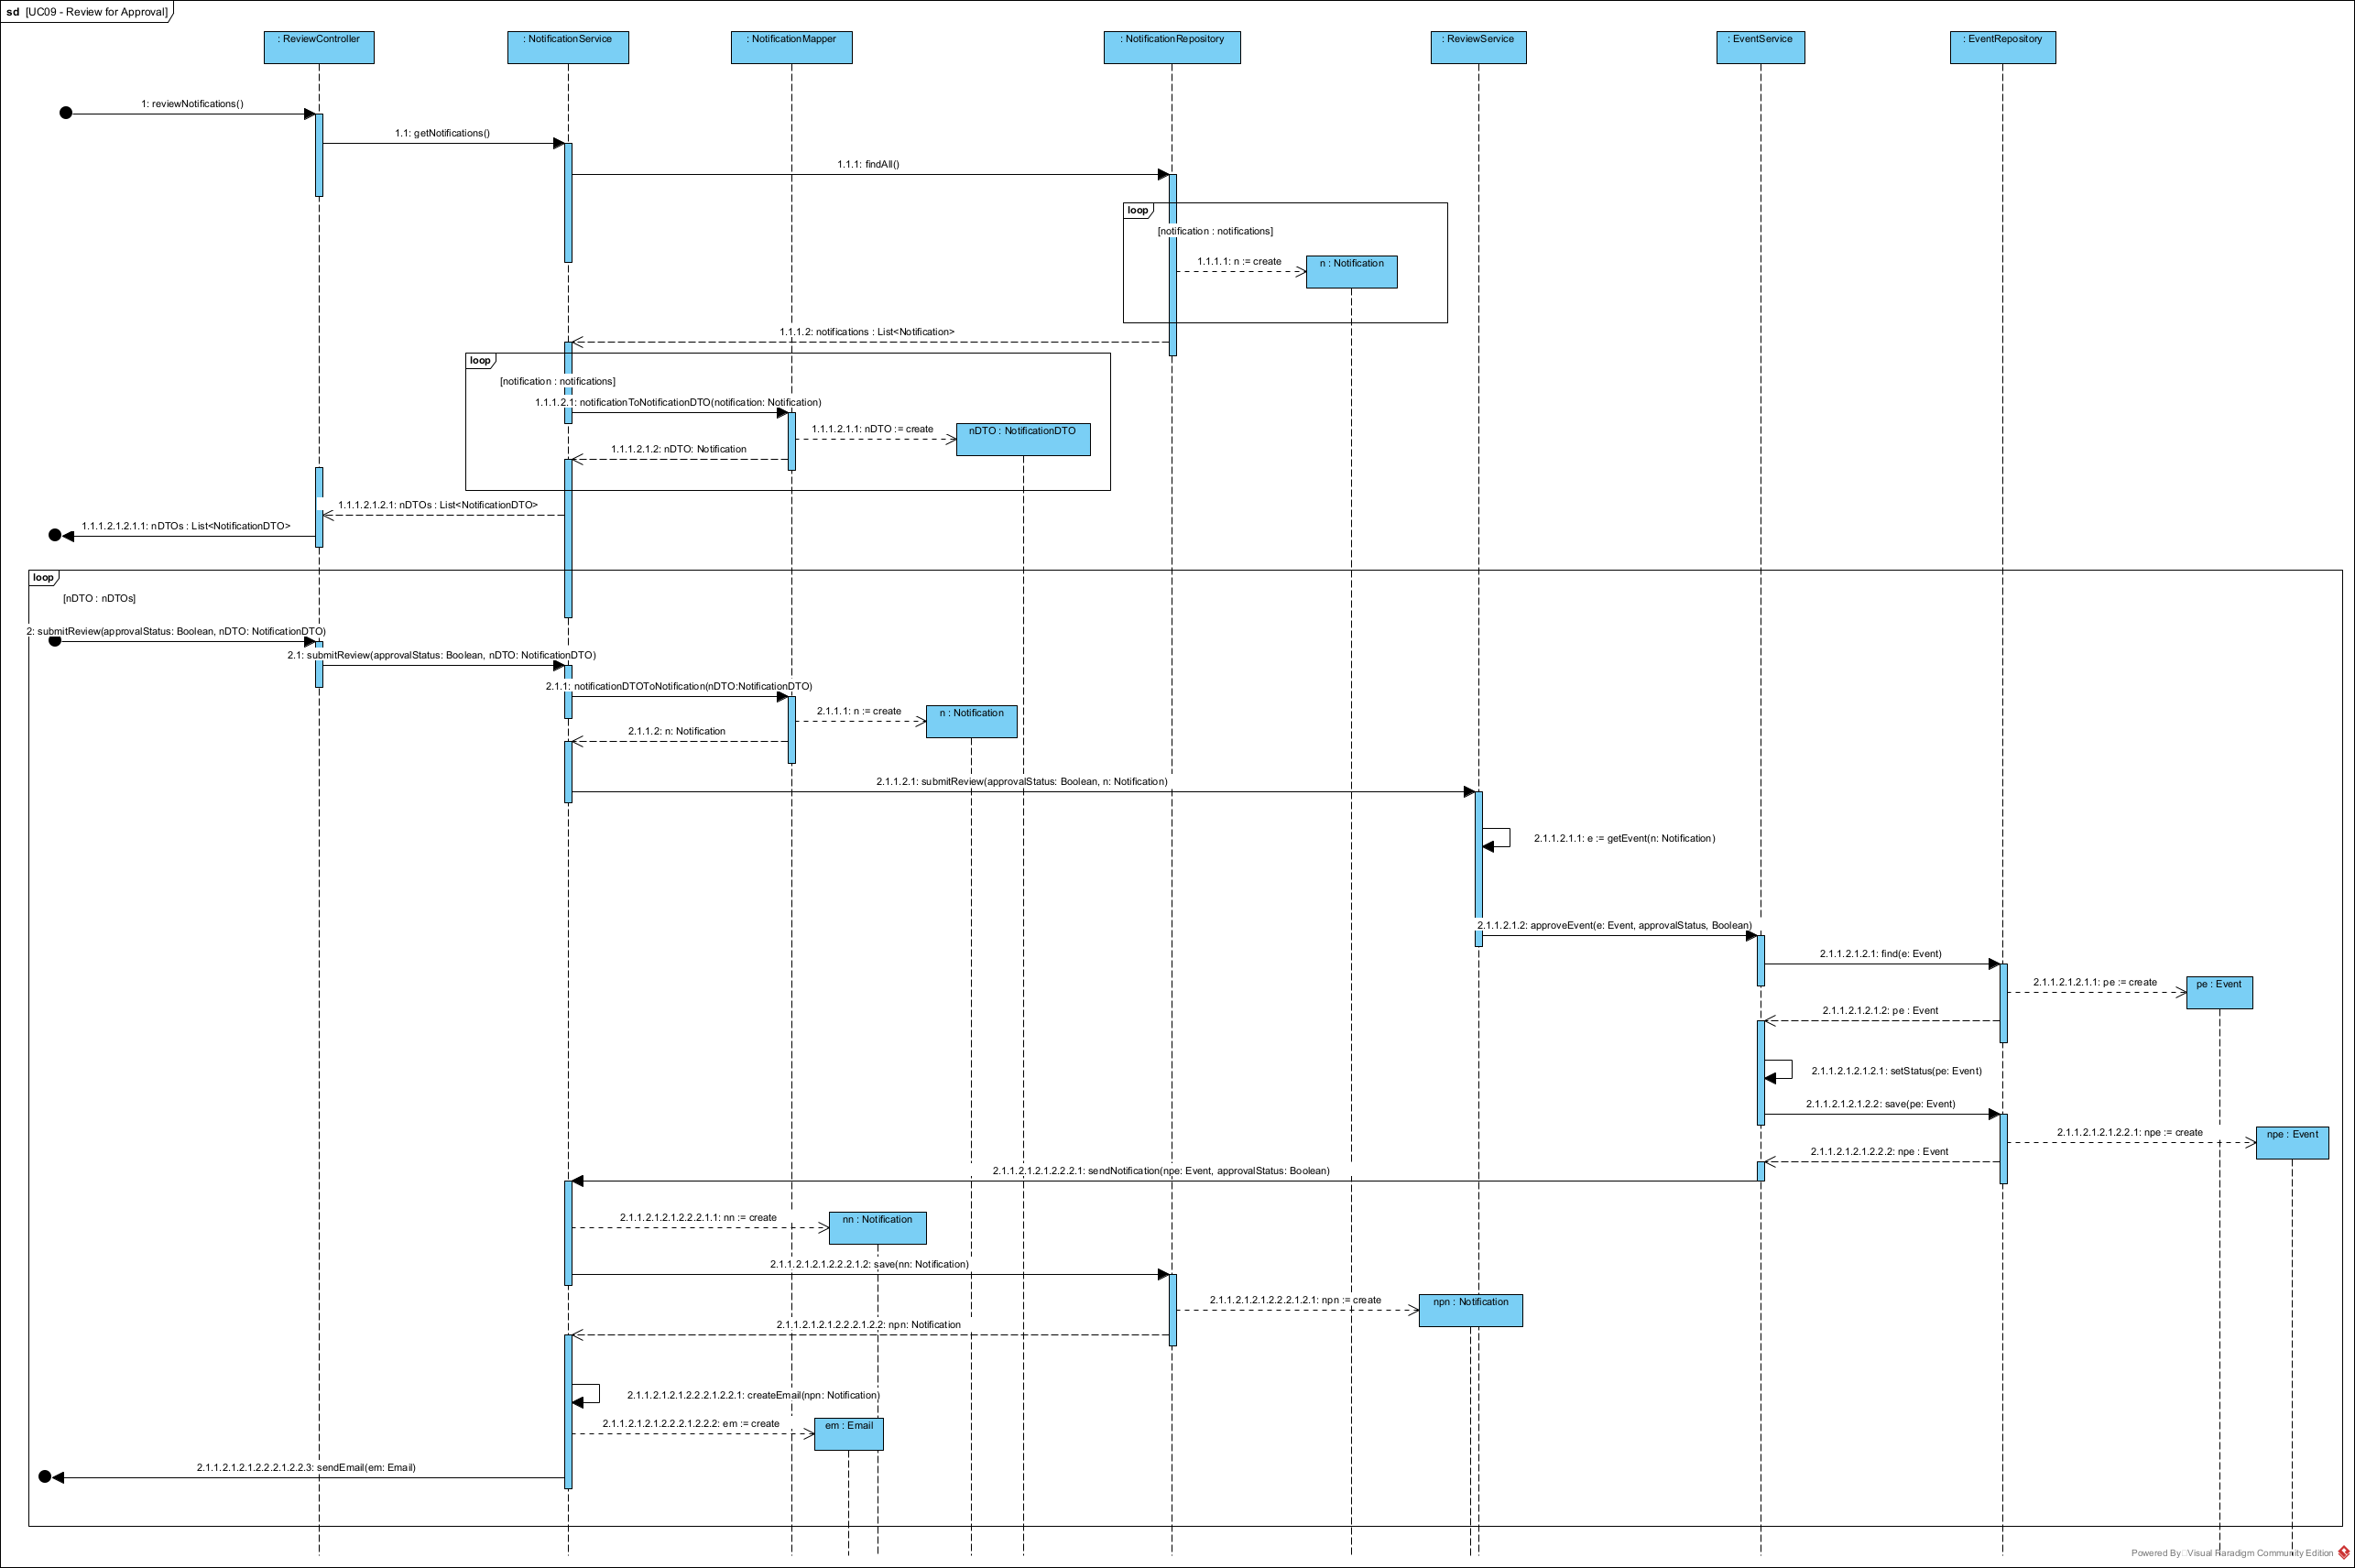
\includegraphics[width=.98\textwidth]{images/SD-UC09-ReviewForApproval.png}
    \centering
    \caption{Sequence Diagram: Review for Approvals}
\end{figure}
\subsection{UC11: Edit post (Pawan Bhandari)}
\begin{figure}[H]
    \centering
    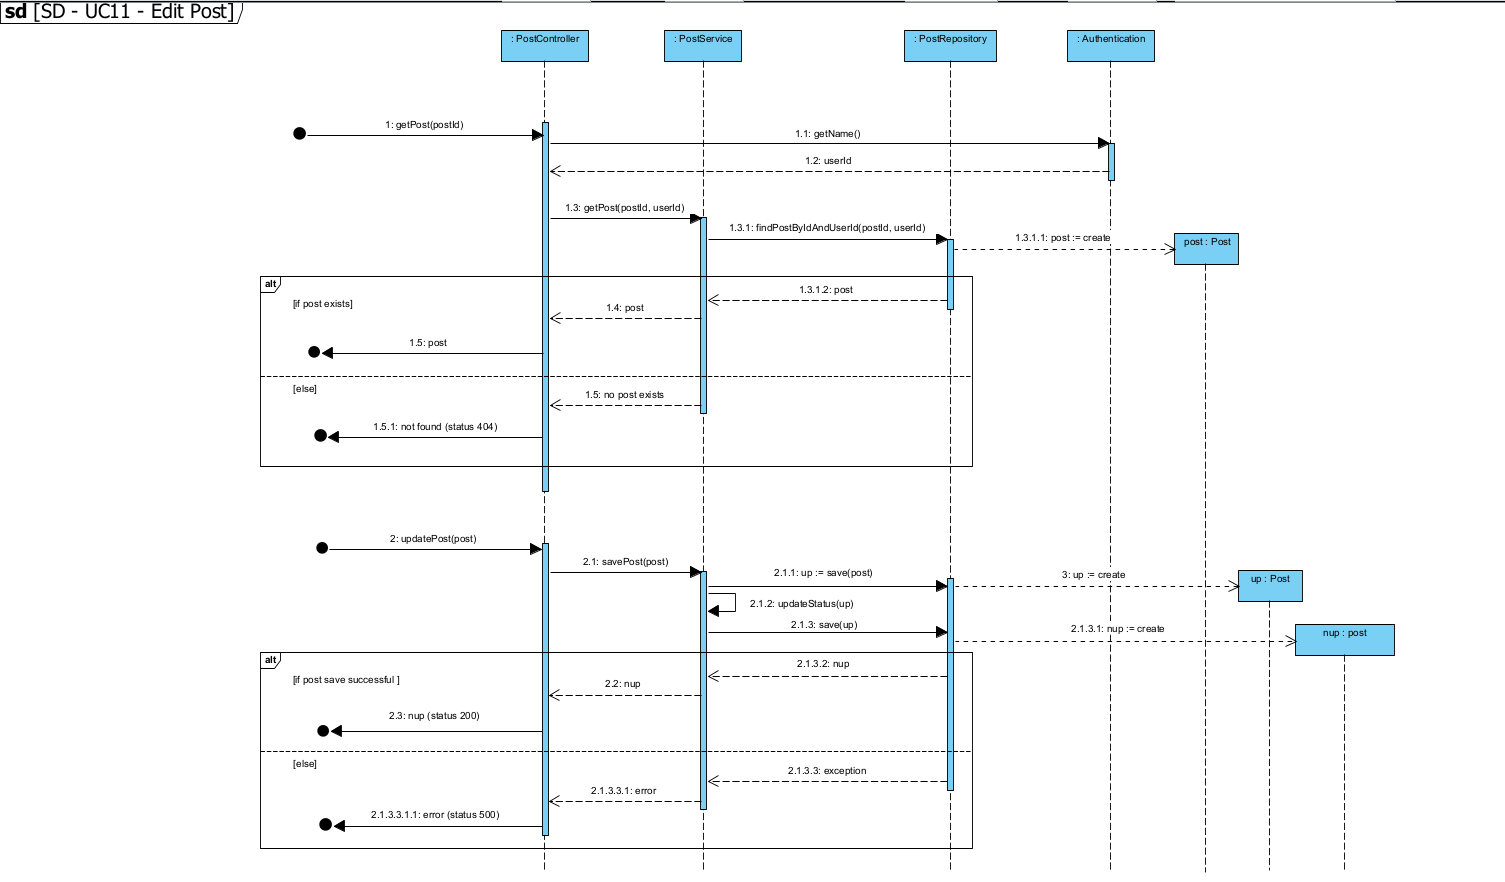
\includegraphics[width=.98\textwidth]{images/SD-UC11-EditPost.png}
    \centering
    \caption{Sequence Diagram: Edit Post}
\end{figure}
\subsection{UC12: Delete post (Pawan Bhandari)}
\begin{figure}[H]
    \centering
    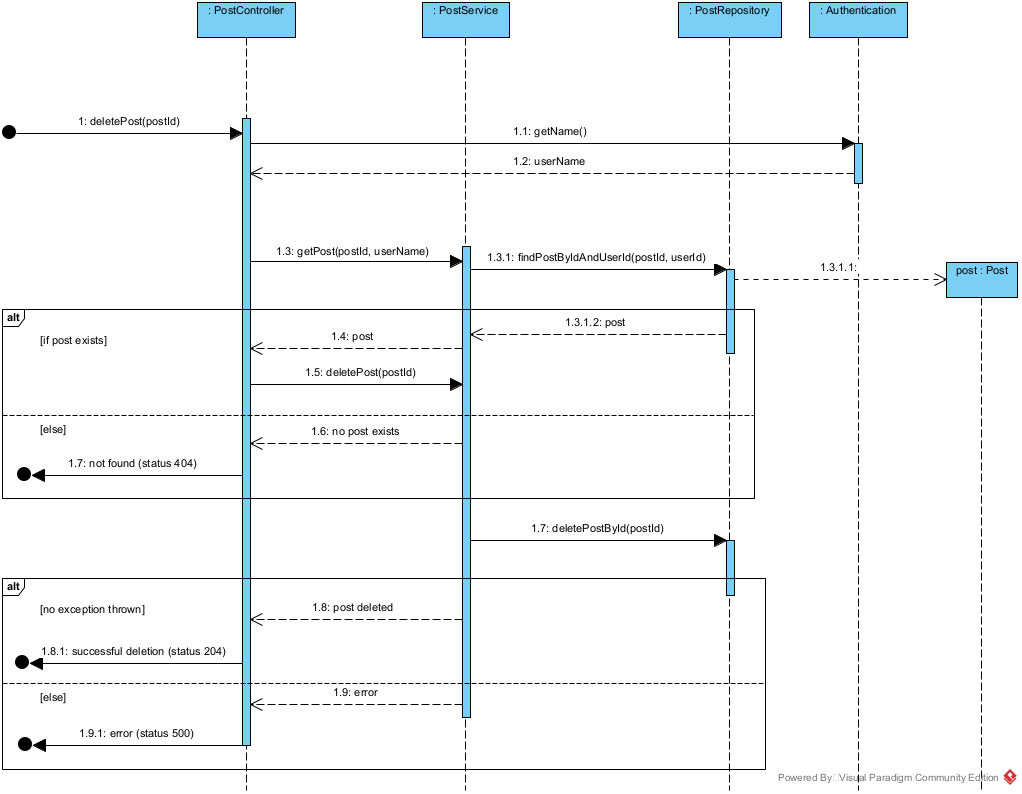
\includegraphics[width=.98\textwidth]{images/SD-UC12-DeletePost.png}
    \centering
    \caption{Sequence Diagram: Delete Post}
\end{figure}
\subsection{UC 5 or 6 or 7: TODO (Sarah Faron)}
\subsection{UC 5 or 6 or 7: TODO (Sarah Faron)}
\subsection{UC 15 or 16 or 1: TODO (Tim Klimpel)}
\subsection{UC 15 or 16 or 1: TODO (Tim Klimpel)}

\end{document}